\section{Card Flow}
\subsection{Overview}
Here we present a vaccine distribution system utilizing physical SafePaths cards and four digitally signed QR code stickers (henceforth termed \textit{Coupon}, \textit{Badge}, \textit{Passkey}, and \textit{Status}). The digital signing of a QR code is simply a secure process of verifying the authenticity of the information contained in the QR code (\cite{crypt}). These QR code stickers are simply QR codes printed onto adhesive stickers that can then be attached to a user’s physical card. 

\begin{figure}[ht!]
\begin{center}
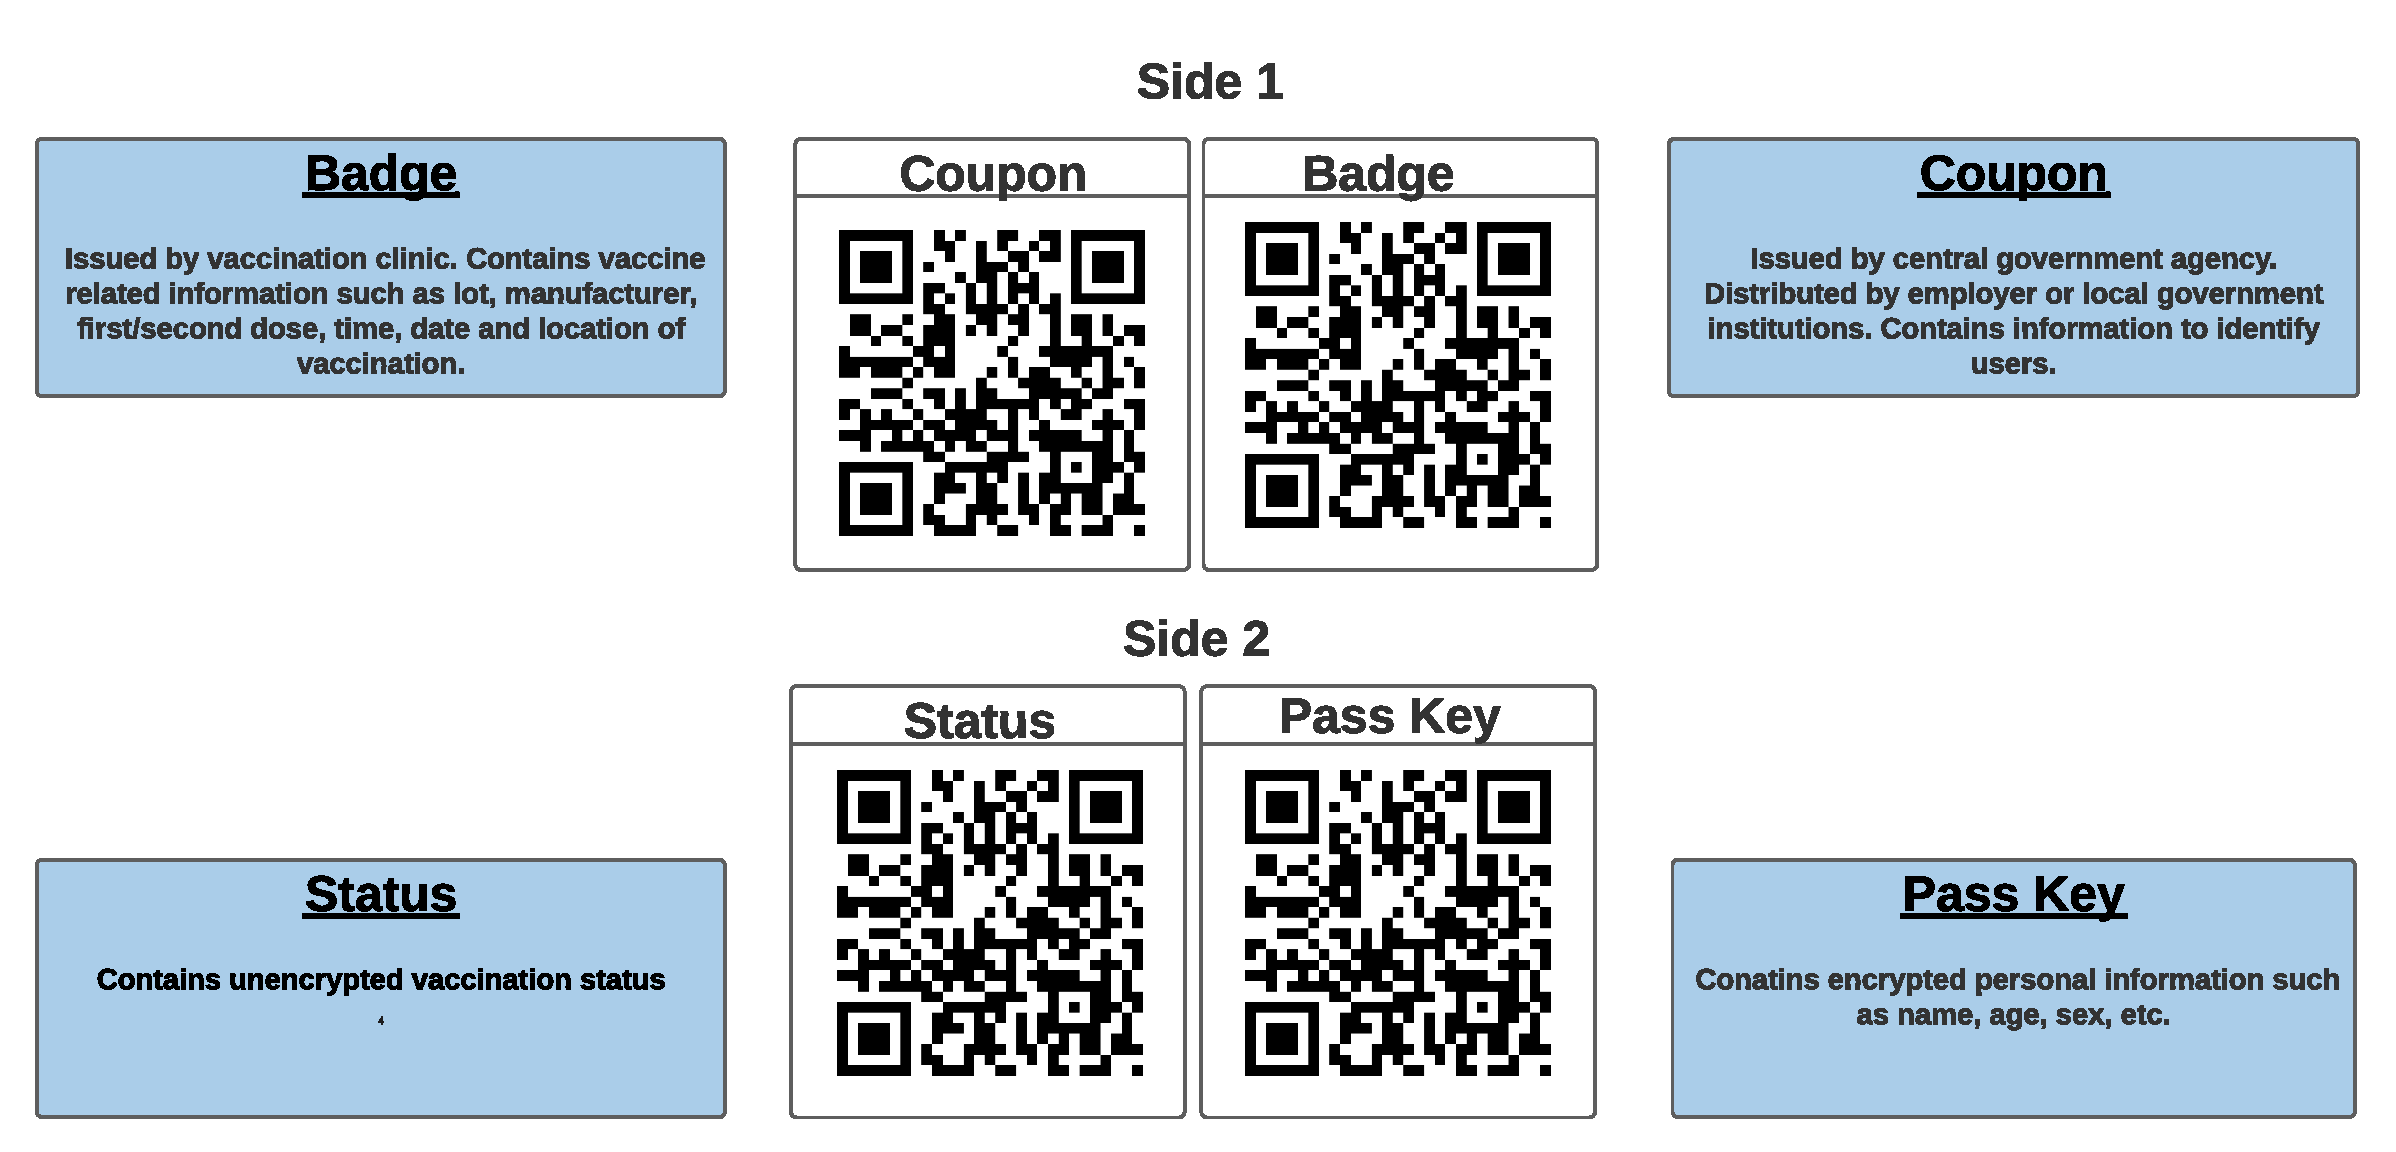
\includegraphics[width=12cm]{images/safepaths_card.pdf}
%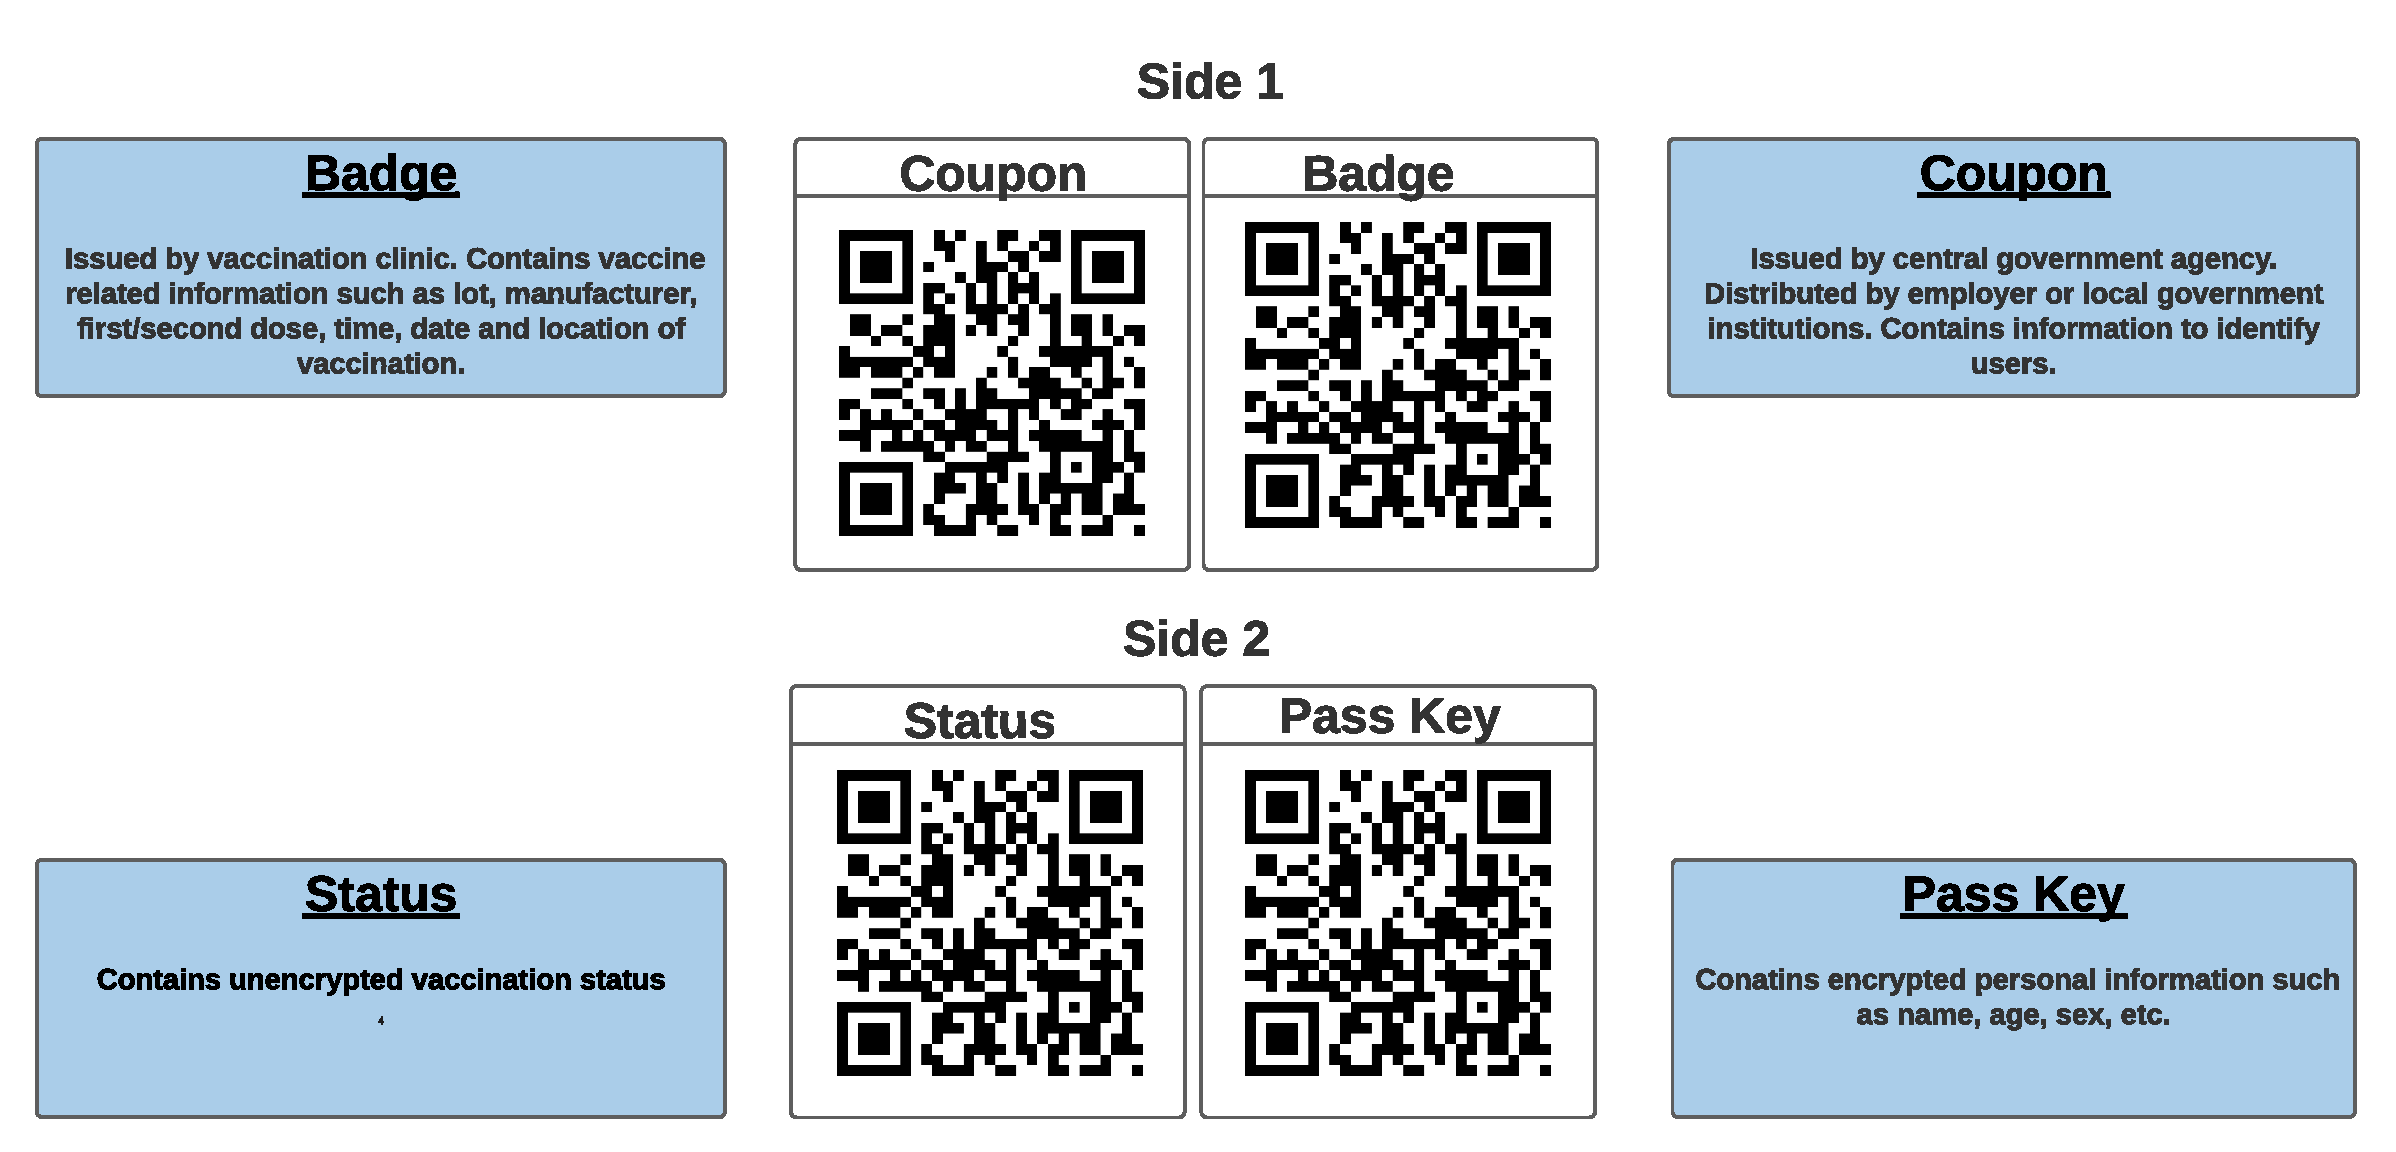
\includegraphics[width=12cm\textwidth,natwidth=610,natheight=642]{images/safepaths_card.pdf}
\end{center}
\caption{The 4 digitally signed QR code stickers (\textit{Coupon}, \textit{Badge}, \textit{Status}, and \textit{Passkey}) present on the SafePaths cards.}
\label{qr-codes}
\end{figure}



\begin{figure}[ht!]
\begin{center}
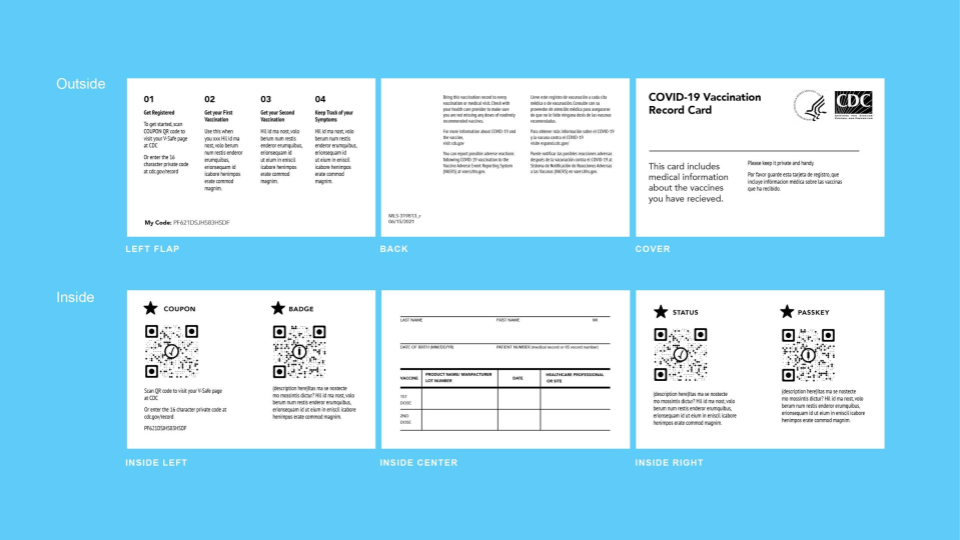
\includegraphics[width=13.5cm]{images/mockup.png}
\end{center}
\caption{MIT SafePaths Card Mockup}
\label{mockup}
\end{figure}
The digital signature of the QR codes take place as below
\textbf{Certificate = (message, signature(messages))}

For each sticker below the message is as follows - 
\begin{itemize}
    \item \textbf{Coupon} = (number, total, city, phase, (age, job, comorbidities/sick))  
    \item \textbf{Badge} = (coupon, dose\_info, Hash(passkey())
    \item \textbf{Status} = ((vaccinated = 0,1,2), Hash(passkey())
    \item \textbf{Passkey} = (name, DOB, salt) \\
    = hash:sj2d8k8hy7j
    
\end{itemize}
\begin{table}[!htb]
\begin{tabular}{|l|l|l|l|}
\hline
\multicolumn{1}{|c|}{\textbf{Name}} &
  \multicolumn{1}{c|}{\textbf{Equation}} &
  \multicolumn{1}{c|}{\textbf{Description}} &
  \multicolumn{1}{c|}{\textbf{Example}} \\ \hline
Coupon &
  \begin{tabular}[c]{@{}l@{}}\{m, sign(m)\} \\ where m = (i, zip code, \\ job type)\end{tabular} &
  \begin{tabular}[c]{@{}l@{}}Coupon code is signed \\ by CDC and indicates the\\  zip code and job type of the \\ receiver\end{tabular} &
  \begin{tabular}[c]{@{}l@{}}\{37, 5000, Springfield, 1B, \\ Teacher\}\end{tabular} \\ \hline
Badge &
  \begin{tabular}[c]{@{}l@{}}\{m, sign(m)\} \\ where m = (dose\_info, \\ coupon, hash(passkey))\end{tabular} &
  \begin{tabular}[c]{@{}l@{}}Badge is available after 2 \\ doses and it gives the \\ information pertinent to \\ the vaccine shot.\end{tabular} &
  \begin{tabular}[c]{@{}l@{}}\{{[}Pfizer, “1st Dose”, \\ 1/1/2021{]}, fe4c2, \\ 3be33c20cc4c85a0c32f7bf5b4\}\end{tabular} \\ \hline
Status &
  \begin{tabular}[c]{@{}l@{}}\{m, sign(m)\} \\ where m = (status, \\ hash(passkey))\end{tabular} &
  \begin{tabular}[c]{@{}l@{}}Contains bare minimum \\ information to prove the \\ user is vaccinated\end{tabular} &
  \begin{tabular}[c]{@{}l@{}}\{vaccinated, \\ 3be33c20cc4c85a0c32f7bf5b4\}\end{tabular} \\ \hline
Passkey &
  \begin{tabular}[c]{@{}l@{}}ID = User\_PII\\ Key = salt\end{tabular} &
  \begin{tabular}[c]{@{}l@{}}Key is the random salt \\ used for increasing the \\ entropy of hashed data\end{tabular} &
  \begin{tabular}[c]{@{}l@{}}\{John Doe, \\ 6363fe744f74ee8f280958\}\end{tabular} \\ \hline
\end{tabular}
\caption{This outlines the four QR codes and what information is digitally signed in it.}
\label{tab:my-table}
\end{table}

Our solution is intended to decouple the health information and personally identifiable information (PII) in this process. Thereby, we are essentially proposing to separate the eligibility of the vaccination from the distribution of it. This way we can have the health information centralised, whilst the PII information decentralised.


\subsection{Vaccine eligibility confirmation}
To accommodate the several-stage vaccination policies that countries have begun to employ, SafePaths cards will be distributed containing one digitally-signed \textit{Coupon} QR code. This would be provided by a central government agency such as the CDC and made available to users either by an employer or local government location. A pseudo random identifier generated for this \textit{Coupon} serves as the identifying information for the user throughout the remaining workflow. This \textit{Coupon} would initially come with  SafePaths cards while the remaining three adhesive stickers must be obtained and placed onto the card following vaccination events.

\subsection{Vaccine administration}
Check-in at a vaccination clinic would require the verification  of a user’s \textit{Coupon}. 

Upon vaccination, the vaccination clinic would create a digitally-signed record of immunization and print it as a QR code on an adhesive sticker. This adhesive sticker (henceforth referred to as the \textit{Badge}) would contain information regarding vaccine lot, manufacturer, and first/second dose information. The \textit{Badge} would also contain information regarding the time, date, and location of vaccination. 

The vaccination clinic would also create a unique encryption key to encrypt the \textit{Badge}. This key, as well as encrypted PII such as name, age, sex, etc. would be stored on a \textit{Passkey} QR code, printed onto a \textit{Passkey} QR sticker. This \textit{Passkey} is required for decryption of PII and in-depth vaccination information (time, date, location of vaccination). 

At this stage, a vaccine recipient would then have \textit{Coupon}, \textit{Badge}, and \textit{Passkey} QR stickers. 


\subsection{Second Dose}
When a user attempts to receive a second dose of a vaccine, the vaccination clinic would  utilize a user’s \textit{Badge} to determine the appropriate vaccine type and dose and the \textit{Passkey} to confirm a user’s identity. Again, the user \textit{Passkey} contains information that solely exists on the physical card carried by a user. Use of this sticker is required to decrypt in depth vaccination information for a patient contained in the \textit{Badge} (location of vaccination, date, etc.). Once final vaccination has been performed, the vaccine clinic would create a fourth and final \textit{Status} QR code sticker for a recipient’s SafePaths card, which would simply indicate whether or not a user has been vaccinated. \textit{Status} would not contain any further information and therefore would be unencrypted.  
\subsection{Record-keeping}
User vaccination records could be linked by anonymized upload to a centralized system using a user’s pseudorandom identifier. The user’s \textit{Passkey}, containing their encryption key that decrypts their PII, would not be uploaded to the CDC without consent. Alternatively, we propose an anonymous record keeping function in our Scanner App section. 
\subsection{Vaccination verification}
Verification of immunization status might be required in various scenarios such as airline travel, return to school/work, etc. Vaccine verification at these venues would follow the receipt of a second COVID-19 dose. 

Information regarding an individual’s vaccination status would be digitally signed by the vaccine clinic onto the \textit{Status} sticker. When scanned, this sticker would provide the verifier with information regarding whether or not an individual has been vaccinated. If further verification of identity is required, the verifier could make use of a consenting individual’s \textit{Passkey} sticker to decrypt the holder’s name. With this method, a user would have multiple levels of information they can share, beginning with vaccination status in the unencrypted \textit{Status} sticker, basic personal information (i.e. name) that must be decrypted using the \textit{Passkey} sticker, and finally full personal vaccination information encrypted in the \textit{Badge}.  

\subsection{Safety and efficacy monitoring}
Short and long-term monitoring of health outcomes would rely on self-reporting. These cards could still facilitate the anonymous information upload by interacting with existing centralized systems such as VAERS or V-Safe while bypassing PII input. All health and symptom information could instead be tied to a user’s pseudorandom ID. We also propose a scanner app solution in the Scanner Flow section that could aggregate symptom reporting and vaccine record data anonymously.  

\begin{figure}[ht!]
\begin{center}
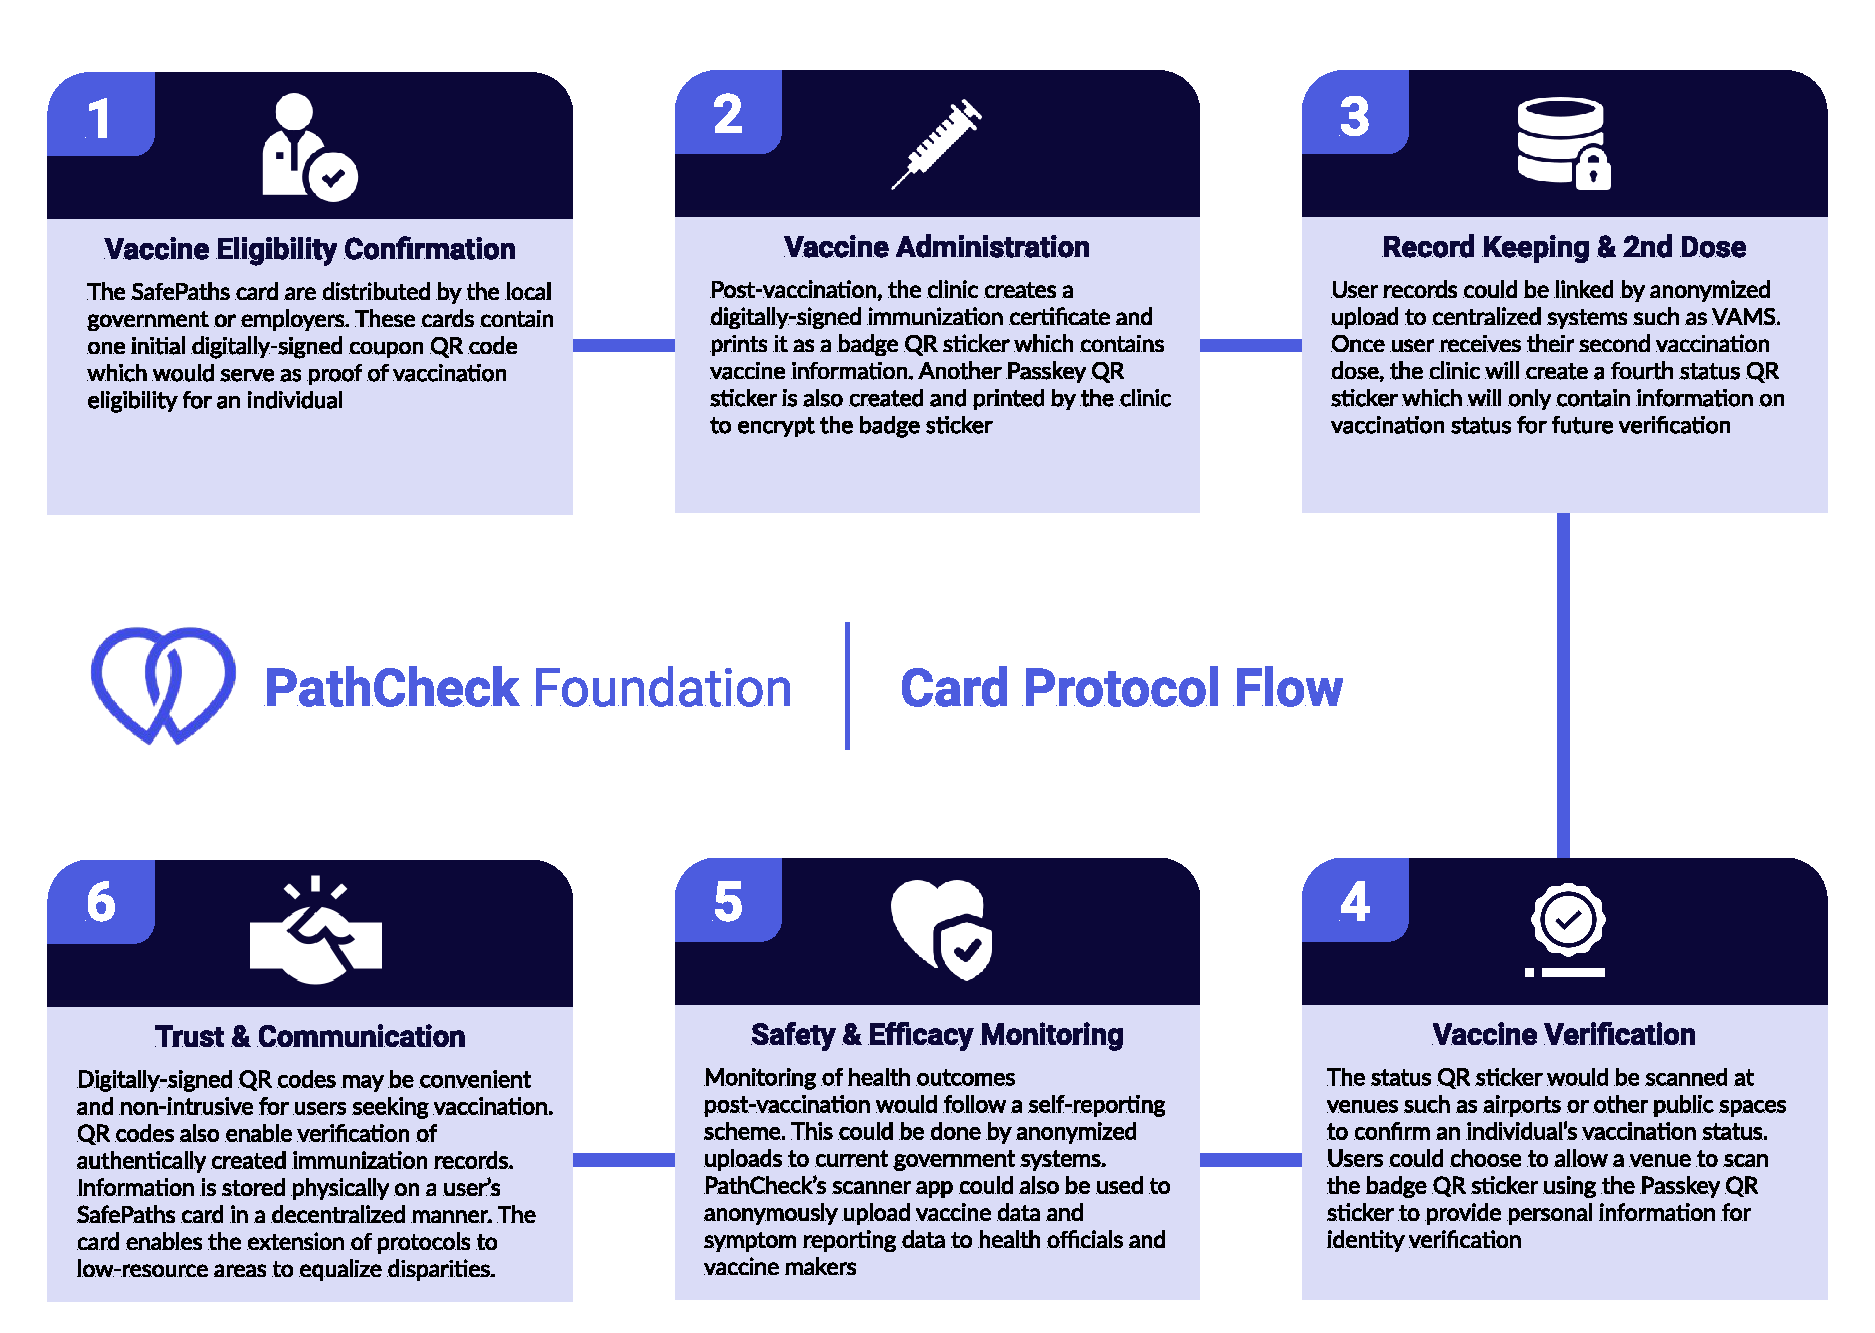
\includegraphics[width=13.5cm]{images/card_protocol.pdf}
\end{center}
\caption{Card protocol workflow diagram.}
\label{card-protocol}
\end{figure}